\documentclass[conference]{IEEEtran}
\IEEEoverridecommandlockouts
% The preceding line is only needed to identify funding in the first footnote. If that is unneeded, please comment it out.
\usepackage{cite}
\usepackage{amsmath,amssymb,amsfonts}

\usepackage{graphicx}
\usepackage{textcomp}
\usepackage{xcolor}
\usepackage{algorithm} 
\usepackage{algpseudocode} 
% Emad Added the bellow packages
\usepackage{todonotes}
\usepackage[inline]{enumitem}

\def\BibTeX{{\rm B\kern-.05em{\sc i\kern-.025em b}\kern-.08em
    T\kern-.1667em\lower.7ex\hbox{E}\kern-.125emX}}
\begin{document}


\title{Distinct Groups on Find Usages}

\author{\IEEEauthorblockN{1\textsuperscript{st} Given Name Surname}
\IEEEauthorblockA{\textit{dept. name of organization (of Aff.)} \\
\textit{name of organization (of Aff.)}\\
City, Country \\
email address}
\and
\IEEEauthorblockN{2\textsuperscript{nd} Given Name Surname}
\IEEEauthorblockA{\textit{dept. name of organization (of Aff.)} \\
\textit{name of organization (of Aff.)}\\
City, Country \\
email address}
\and
\IEEEauthorblockN{3\textsuperscript{rd} Given Name Surname}
\IEEEauthorblockA{\textit{dept. name of organization (of Aff.)} \\
\textit{name of organization (of Aff.)}\\
City, Country \\
email address}

}


% \author{
% \IEEEauthorblockN{Emad Aghayi}
% \IEEEauthorblockA{\textit{Department Of computer Science} \\
% \textit{George Mason University}\\
% Fairfax, VA \\
% eaghayi@gmu.edu}
% \and
% \IEEEauthorblockN{Aaron Massey}
% \IEEEauthorblockA{\textit{Department Of computer Science} \\
% \textit{George Mason University}\\
% Fairfax, VA \\
% amassey5@gmu.edu}
% \and
% \IEEEauthorblockN{Thomas LaToza}
% \IEEEauthorblockA{\textit{Department Of computer Science} \\
% \textit{George Mason University}\\
% Fairfax, VA \\
% tlatoza@gmu.edu}
% % \and
% % \IEEEauthorblockN{3\textsuperscript{rd} Given Name Surname}
% % \IEEEauthorblockA{\textit{Department Of computer Science} \\
% % \textit{George Mason University}\\
% % Fairfax, VA \\
% % email address or ORCID}
% }

\maketitle

\begin{abstract}
Developers face many challenges when trying to understand large codebases. In particular, they have difficulties in understanding the context of how various internal classes, objects, or methods are used in the codebase. We sought to better understand these challenges by conducting a think-aloud user study with 6 participants. The results of the think-aloud experiment highlighted that developers spend considerable time learning to use internal code artifacts. The result also showed developers use the Find Usages/References feature of IDEs to understand code by example. The results of Find Usages can be long tail of results that developers find difficulty mentally parsing. We also found that find usage/reference results' would contain duplicate examples in disparate locations in the UI, adding to the difficulty of parsing. Based on the think-aloud study, we hypothesized that removing duplicate examples and grouping similar examples together would reduce the excise in using the Find Usages/references tool. We designed and implemented a plugin for IntelliJ IDEA that manipulated result of Find Usages and grouped them based on their similarity. After that, we conducted a controlled experiment with 12 more participants to evaluate our approach. Results showed that this aggregation of Distinct examples is useful.
\end{abstract}

\begin{IEEEkeywords}
Code navigation, information foraging, Find Usages, Find References, large Codebase
\end{IEEEkeywords}


\section{Introduction}
Developers are facing many challenges every day for understanding codebase. They have difficulties in understanding the context of how members are used, for instance, how object A is used in the codebase. Another daily issue is navigation from one statement other to task-related code. Sometimes developers want to go through related statements to understand the codebase. Also, they are facing challenges to answer questions about how a change affects callers when developers want to change an artifact before changing that they check the side effect of that change. They go through the codebase and evaluate the effect of change on them. There exist multiple approaches for better support of structural navigation.\par
During programming tasks, it is not uncommon for a developer to use an object or routine they were previously unfamiliar with. A programmer could also be unfamiliar with how a resource is used within a codebase versus the resource itself. Typically, programmers scour the web for documentation or examples~\cite{brandt2009two}. However, this is not an option for closed source code, forcing developers to rely on internal documentation and examples. Since this may be non-existent or worse (incorrect), example code is a more reliable information source for programmers. The industry-standard approach for finding examples is the Find Usages/References tool. However, when large numbers of references are returned from this tool, it can be not very easy for users to parse the results visually .\par
We conducted an exploratory study to find are challenges of understanding codebase while developers are trying to use the Find Usages feature of IDEs. During an exploratory user study, participants would get overwhelmed with the number of results and that instead of investigating more usages, participants would select a single usage and use it as a particular example for quite some time before moving on to find other potentially better examples.
We hypothesized that some intelligent aggregation of the results would make these results easier to parse, thus improve programmer task time.\par
Based on the result of exploratory study, we designed and developed a plugin for addressing the issues that we found.The plugin manipulated  result  of  find  usages and  grouped  them  based  on  their  similarity.  After  that,  we conducted  a  controlled  experiment  with  12  more  participants to  evaluate  our  approach. At the end of the study we conducted interview with particiapnts of both groups to get more data. Results  showed  that  this  aggregation of  Distinct  examples  is  useful.\par

In the rest of the paper, we first provide a background on code navigation, code edit, and code clone, then we general information about exploratory study we conducted on Find Usages feature of IntelliJ IDEA. Then we discussed about our approach. After that evaluation of our approach is described. Finally, we conclude with a discussion of limitations as well as opportunities and future directions.

\section{Relate Work}
Developers are using code navigation in their daily activities. For instance, they want to want to understand what a method does or when it is called or want to understand how to reuse a function by finding examples of code snippets. They investigate source code. Navigating in source code is described in information foraging theory~\cite{pirolli1999informationforaging}. In software engineering, this theory usually modeled as call graphs. Methods are nodes, and function invocations are edges. Developers have challenges in traversing the call graph in code navigation~\cite{albusays2017interviews}. Navigating and re-finding place of the code that had already been visited was frequent, difficult and distracting~\cite{ko2005eliciting,deline2005towards}.\par 

Tools are trying to help developer to be more productive in the code navigation. These tools are grouped into three categories. The first category is structural relationship traversal. These tools find starting point then traverse relationships to find other related code locations~\cite{karrer2011stacksplorer,augustine2015field,latoza2011visualizing}. Another category is recommender tools. Based on history developers did on similar tasks, they predict relevant elements~\cite{zimmermann2005mining,deline2005easing}. Task context navigation is the last category of code navigation tools. They make it easier to navigate back and forth between task context elements~\cite{ko2006exploratory}. Although there exist several tools for code navigation, code navigation is still challenging for developers~\cite{albusays2017interviews}. 

A common way to edit code is by copying existing code, called code clones~\cite{codeCloneDetection2019}. Sometimes code clone is bad, but there exist many situations that code clone is fine. Developers, because of reasons like basic template, design patterns, or reuse of the definition of specific behavior, use code clones~\cite{kim2004ethnographic,kapser2008cloning}. There exist many tools for detecting code clones in codebases~\cite{bellon2007comparison}.\par 

There is a plethora of research on information foraging and improving learning by examples~\cite{brandt2009two}. There is also much work in code clones code clone clustering~\cite{codeCloneDetection2019}. As far as these authors are aware, this is the first time work on code clones, and their clustering has been used to help forage for examples within a codebase. Typically code cloning is used to infer duplicate code snippets for refactoring or patching. Researchers have attempted to take relevant pieces from each of these fields, and it is this combination of parts that is the contribution~\cite{kapser2009toward}.\par


Find a similar code in a codebase is one code reuse strategy~\cite{rosson1996reuse}. Developers looking for examples of how to use specific methods or objects~\cite{stylos2006mica,umarji2008archetypal}. Opportunistic developers more likely to use example code rather than systematic developers. There exist techniques for supporting reuse, for instance, IDEs has searching feature that enables developers to search for example across the existing codebase, or IDEs has feature for fining right sequence of methods to complete some tasks that developer already started.\par

Developers, when they write or edit code, they might come across code element that they want to change or delete. Before they make changes, they look where the code element is used and how it affects the codebase. \textit{Find Usages} feature in Jetbrains IDEs and \textit{Open Call Hierarchy} feature of Eclipse Provided this ability for developers. Results of Find Usages are listed in window in Jetbrains IDEs that developers are going through the results to find the desired usage or understand the codebase. 
\todo[inline]{add challenge of Find Usages}
\par



\section{Challenges and Benefits of Understanding Codebase}
We conduct a think-aloud study to understand better current practice and the challenges developers face using existing approaches. The study was in-person, and their interaction and thoughts were recorded. Researchers vocally recorded the process while asking the participant to think-aloud while conducting the study. The participants were allowed to ask for hints or questions or clarifications, but we must not give answers.
We were not looking for successful implementation. We were looking for what developers think about the Find Usages interface, without coaxing the answers we may want out of them.
We recruited four participants (P1, P2, P3, P4), two female and two male. The first participant was a graduate computer science student at George Mason University. The remaining three participants were working as a software developer in the industry, two of them had experienced less than one year, but one of them had more than four years of experience in the industry. We designed two tasks for the study. In the beginning, the tasks were piloted with the graduate student participant to make sure the tasks are designed correctly or not. At the and of study, we asked participants to respond to a survey for collecting their experience. In that survey, we asked them 1)What challenges did they experience related to finding a method, variable, or anything. 2)What challenges, if any, did they experience as they tried to begin work l on these tasks? 3)What challenges, if any, did they experience related to understanding and working with the provided codebase? 4) What challenges, if any, did they experience related to their productivity? 

\subsection{Tasks}
\label{tasks}

The first task was a warm-up for using a Find Usages tool for code comprehension. The codebase that participants worked on it was Google Guava (772,475 LOC), an open-source set of standard libraries for Java. We chose this library because we thought it is standard and is large enough. We gave the participant a zip file that contained the Guava and asked them to qualitatively describe the range of integer inputs given to the two methods. We gave participants to work on firs task on any IDE that they are more familiar with. Time of the first task was 10 minutes.\par

Since we also wanted to understand the behaviors of developers when they are trying to change a codebase, we designed second task for developers. The codebase that we chose for this task was FlyingSaucer, pure Java library for rendering XML, XHTML, and CSS. It was a large codebase 99,000 LOC. We removed statements that create PDF from the codebase, then asked participants to implement functionality to produce “success.pdf.” We added a constraint on the task. Participants should treat code as closed source code, meaning they cannot find Javadocs online or look for online code examples, but they were free to choose any IDE for accomplishing the task. The study was in person, and it lasts 50 minutes for each participant. 

\subsection{Results of Exploratory Study}


We collected data from the interaction of developers while they were working on both tasks. During the first task, participants clicked through multiple usages trying to understand how certain common arguments to methods were called. We have participants a maximum of 10 minutes to feel like they had become comfortable with the Find Usages tool. Participants completed task two in 49, 20, 42 minutes. Two participants had a problem with the size of the codebase.
\begin{quote}"Overwhelmed by the amount of code." - (P2) \end{quote}
\begin{quote}"Large codebases are my biggest fear." - (P4) \end{quote}
3 of 4 did not know about the Find Usages feature, which was interesting. We gave them information and train them what is Find Usagesfeature and how they can use it. One of them Used the term "implemented" to mean "usage" frequently. In some cases, participants did not have a strong evidence or reason for understanding the codebase. They were trying to use their feeling. 
\begin{quote}"I donot know how .layout() is used but I am going to use it because it's in this code" - (P2) \end{quote}
\begin{quote}"I feel like this [.layout()] should just work, I hope!" - (P4) \end{quote}

Tasks that we defined looked was similar to what they are doing in their job in the industry. 
\begin{quote}
"Not out of the ordinary [from regular industry/work experience] but still a bit overwhelming"- (P2)
\end{quote}
\begin{quote} "This is just like my job" and "I do this at work all the time, no one knows how anything works but we see how things are used"
- (P3)
\end{quote}
The codebase that we gave participants included unit tests. The interesting thing was that participants were using these unit tests to figure out how methods are invoked and what are the possible input arguments for those methods. They primarily utilized tests as examples. Participants sticks to the specific test case, and usage found, do not go looking for others much until it gets too complex of a usage.

\begin{quote} "Tests are a good example of uses." - (P3)\end{quote}

The similarity of Find Usages results was a severe issue for the participants since the codebases were reasonably large. The problem is shown in Fig.~\ref{fig:usege}. The IDE was returning many results, which was challenging for participants to extract useful information for undressing the method or object. When doing find usage, much code looked similar, and it was difficult for the participant to parse for participants. Also, this problem was severe when the method they tied to get Find Usageswas complex and had complicated call graphs.

\begin{figure}
    \centering
    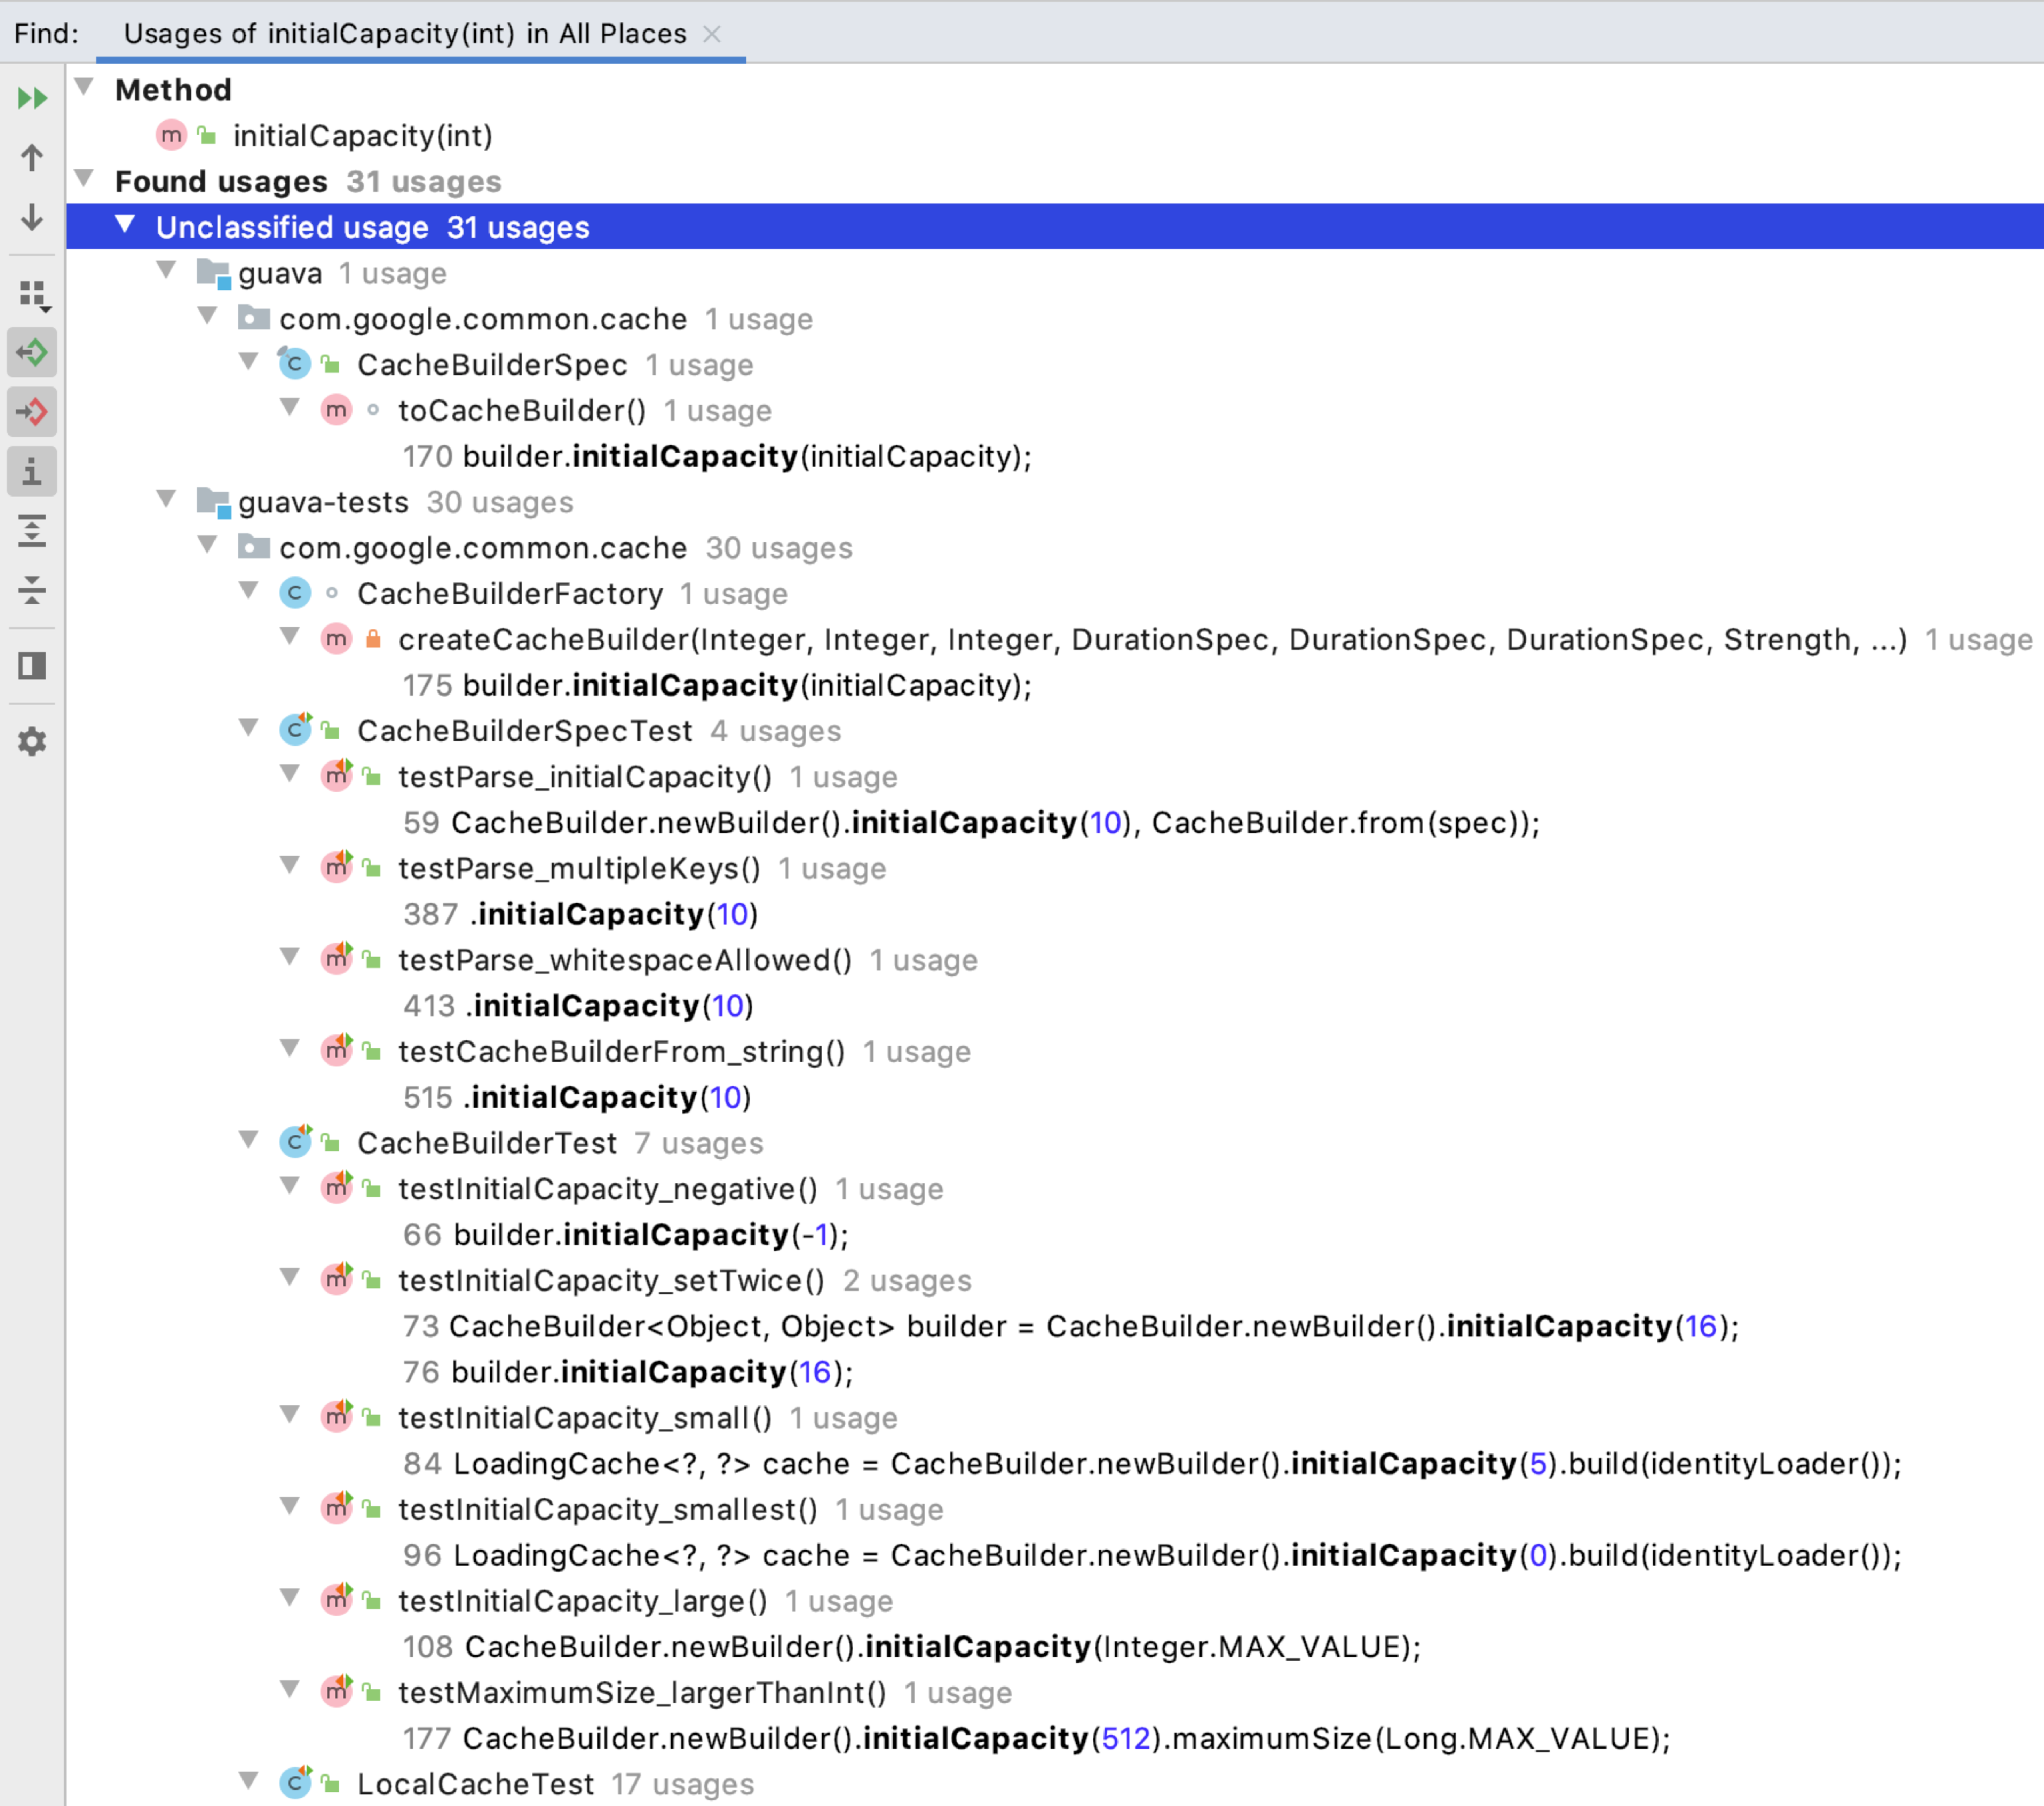
\includegraphics [width=\columnwidth,keepaspectratio, clip]{figures/challenge}
    \caption{It depicts result of regualr Find Usages of IntelliJ IDE. The result window shows there exist 31 usages of the "initCapacity" method. Developers have to go through all of 31 results and also use a pen and paper to find the possible inputs for this method. In this 31 results many of them set same input values of this method, for example 10 is repeated multiple times. This duplicate result is annoying and time consuming for Developers. 
}
\label{fig:usege}
\end{figure}

\begin{quote}"There were a ton of methods and usages that were really similar and it was a lot to put together"- (P4)\end{quote}
\begin{quote}"I had difficulty finding usages with low complexity of calls and uses"- (P4)\end{quote}

Another typical behavior was that participants were Scrolling quickly through usages because the surrounding code was not making calls she wanted to make. Participants occasionally navigated to unhelpful usages that took time. A surprising behavior as participants focused on the first result of Find Usage, they copied the first usage, then paste it into the place they want to implement and tried to change it in the way they want. The confusing thing about Find Usages is happen when a method is overloaded. Participants had difficulty migrating to the correct Find Usages because of overloaded methods.


\section{Find Distinct Usages}
Result of the think-aloud study revealed there exist challenges in using Find Usages feature, participants overwhelmed with tons of usage, and they spent much time in going throw many of them for understating the codebase. We brainstormed on the results and came up with the idea that the refining result of Find Usagesmight help developers and increase their productivity. In order to design a better tool for addressing the issues, we must understand what is going on in the developers' world and understand how our tool can make the developers' productivity higher. Therefore, we summarized research findings into storyboards. After that, we designed a plugin for IntelliJ IDEA that refines the result of the Find Usages feature. It aggregates the results and shows the only relevant results. Relevant results likely depend on a measure of sameness.\par
The basic idea behind Find Distinct Usages is to group results from a standard Find Usages/References IDE operation based on each result's surrounding code. Our approach is to group usages found by the IntelliJ IDEA usage finder and group them based on similar ASTs while presenting the result to the user. Our comparison leveraged the Gumtree Spoon AST Diff framework, where we measured the resulting differing and matching nodes from an object representing the diff. A general overview of our approch is shown in Fig.~\ref{fig:general} 

\begin{figure*}
    \centering
    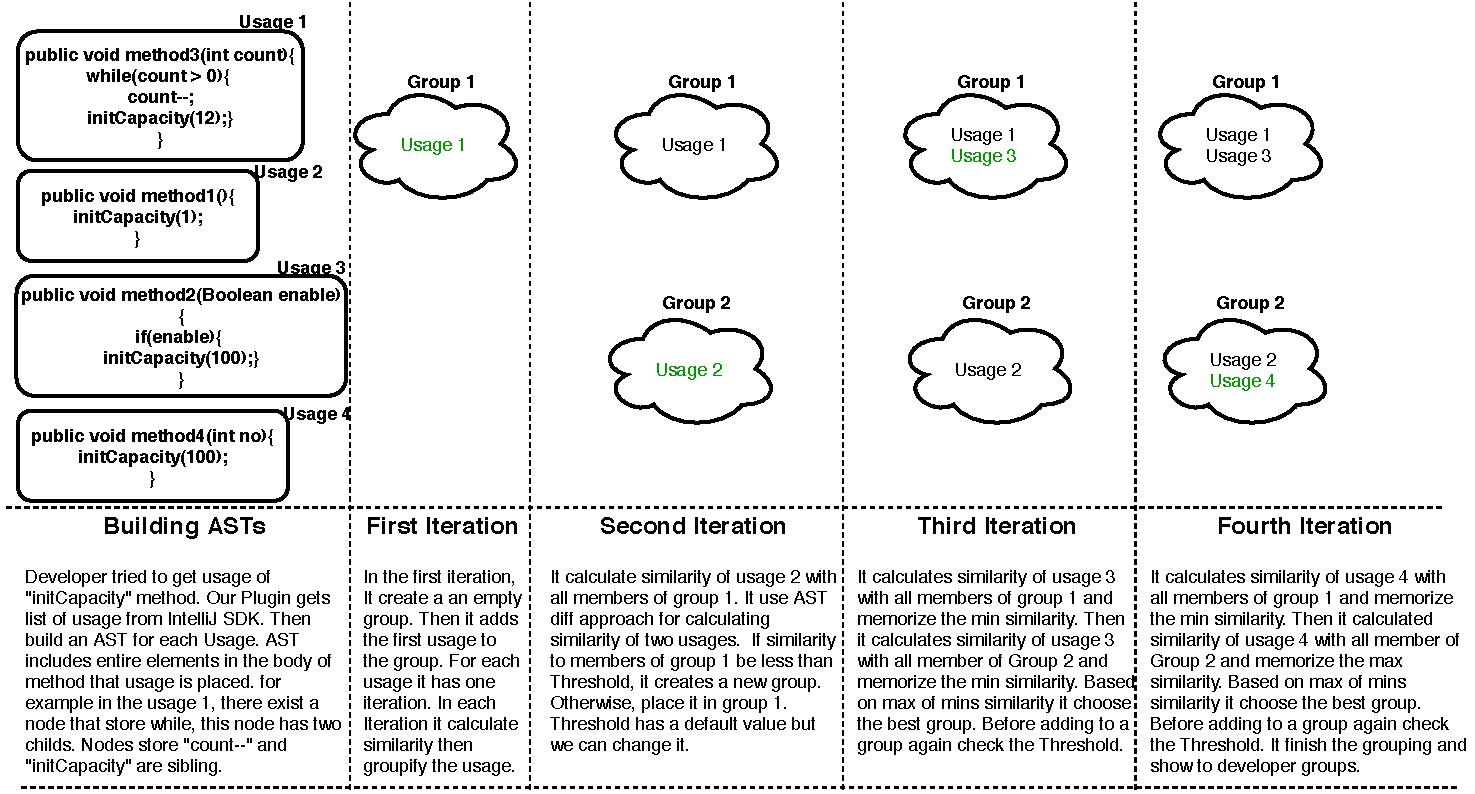
\includegraphics [width=\textwidth,keepaspectratio,clip]{figures/generlView.pdf}
    \caption{This figure depicts how the Find Distinct Usages works. I collect usages and create an AST for each usage. Then based on similarity and threshold it decides to assign it to a group. }
\label{fig:general}
\end{figure*}


\subsection{User Interface} 

Because the adoption of new methodology and new tool can be onerous to programmers~\cite{adaption2002}. We extended the existing Find Usages interface of IntelliJ IDEA by adding additional usage groups that contained usages with similar code. Since each user group contained usages that were surrounded by similar code, we hypothesized the usages would be in similar contexts, implying more information about the usage. So a user could inspect one usage within a usage group and gleam that the other usages within that group were similar and move on to another usage group depending on their task. The task we associate this tool with is finding and parsing a large variety of usages while seeking examples of an internal API.

\subsection{Usage Grouping Back-end} 
Usages were grouped based on similar code within the usage's containing method code block. Logic of the back-end is depicted in Fig.~\ref{fig:flowchart}. For every usage, IntelliJ IDEA calls our aggregate usage method, which returns a reference to a particular Usage Group. An internal IntelliJ IDEA object representing groups of usages. We compare the given usage with all other usages in all existing Usage Groups. We consider the given usage to be a part of a usage group when it has a guaranteed minimum threshold of similarity with every abstract syntax tree (AST)  associated with that Usage Group. If all the Usage Groups have minimum similarities that do not meet the threshold, then we create a new Usage Group with the supplied usage and then return that Usage Group. \par
\begin{figure}
    \centering
    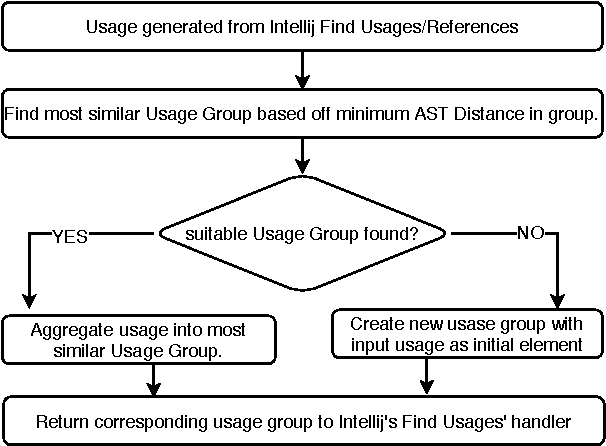
\includegraphics [width=\columnwidth,keepaspectratio, clip]{figures/flowchart}
    \caption{Flowchart shows how the back-end of Find Distinct Usages work. }
\label{fig:flowchart}
\end{figure}

The back-end has three main parts. The first part is an algorithm(see Algorithm1) tries to find minimum similarity between the usage that we want to grouping and all other members of a group. It uses the AST diff formula (\ref{equation1}) for calculating the similarity.\par

\begin{algorithm}
\label{algo1}
    \caption{Minimum Similarity in a Usage Group - minSimilarity($x$, $G_{i}$)} 
    \begin{algorithmic}[1]
    \State Given a Usage $x$ and a Usage Group $G_{i}$
    \If{$G_{i}$ = null}
    \State return  $-\infty$
    \EndIf
    \State $minSimilarity$ $\leftarrow$ $\infty$
    \For{each usage $u_{i}$ in $G_{i}$}
    \State $minSimilarity$ $\leftarrow$ min($minSimilarity$, similarity($x$,$u_{i}$))
    \EndFor
    \State return $minSimilarity$
    \end{algorithmic} 
\end{algorithm}

The second main part is algorithm that tries to find the most similar group for the usage that we want to categorize it, Algorithm 2. This algorithm iterate over all groups and call Algorithm~\ref{algo1} to find the most similar group. At this point we know which group is the most similar to the usage that we want to categorize. But we need to consider similarity Threshold. For example we might choose \textgreater 90\% means very similar, \textgreater 70\% means similar, \textless 40\% means not so similar. Finding an appropriate threshold is critical. A small threshold involve many dissimilar usages and a large threshold might lead to a few results~\cite{deng2013top}. We chose a constant for the similarity threshold of approximately 88\%. There is no real justification for this example besides it working well with an example. In next step our algorithm compare the minimum similarity that it calculated with the threshold and based on decide to create a new group or add the usage to the most similar group. 

\begin{algorithm}
\label{algo2}
    \caption{Find Corresponding Usage Group} 
    \begin{algorithmic}[1]
    \State // Given a Usage $x$ \& a set of Usage Groups $G$
    \State $mostSimilarGroup$ $\leftarrow$ $null$
    \For{each Usage Group $G_{i}$ in $G$}
    \If{minSimilarity($x$, $mostSimilarGroup$) $<$ minSimilarity($x$, $G_{i}$)}
    \State $mostSimilarGroup$ $\leftarrow$ $G_{i}$
    \EndIf
    \EndFor
    \State // Given some similarity threshold $T$
    \If{minSimilarity($x$, $mostSimilarGroup$) $<$ $T$}
        \State // Create new usage group and modify $G$.
        \State $G_{new}$ $\leftarrow$ newUsageGroupWithInitialMember($x$)
        \State $G$ $\leftarrow$ $G$ $\cup$ \{$G_{new}$\}
        \State return $G_{new}$
    \EndIf
    \State addToGroup($mostSimilarGroup$, $x$)
    \State return $mostSimilarGroup$
    \end{algorithmic} 
\end{algorithm}


The last and most important part of our plugin is AST diffing approach. The basic problem in similarity of usages was finding a degree of similarity between two usages. The easiest approach is string distance algorithms such as Hamming distance and Levenshtein distance. Each element in the code can be placed in an AST. For exmaple a \textit{Foreach} is an statement which is child of method, the method is child of class. Another simplification is decreasing the usage to the lowest level which is leaf of AST. In our first iteration of creating the plugin we used string distance, and considered only the leaf node of the AST that contains the usage. After several piloting we found this naive approach is not fine. Therefore, we made two major changes in the first approach. The first change was that we increased the scope of usage to the entire body of the method that usage placed, in fact we tried to find similarity among sub-trees instead of leaf nodes of ASTs. Therefore, we increased the scope and consider the entire body of the method that usage places in as a sub-tree. Rather than comparing sub-trees for exact match, we compated sub-trees similarity based on multiple parameters~\cite{baxter1998clone}.The similarity used a threshold that specify how similar to sub-trees should be. The formula that compute similarity is:
\begin{equation}
Similarity = 2 \times S  \div (2  \times S  + subAST1 + subAST2)
\label{equation1}
\end{equation}

where $S$ is number of shared nodes between two sub-trees, $subAST1$ is number of different node in sub-AST 1, and $subAST2$ is number of different node in sub-AST 2. \par
Another modification was changind string distance algorithms to a more poweful algorithm. We used GumTree~\cite{baxter1998clone,DBLP:conf/kbse/FalleriMBMM14,falleri2014fine}, which leverage the GumTreeDiff algorithm. We chose this algorithm because GumTreeDiff is focused on fine-grained differentiation that is more sensitive to a programmer~\cite{falleri2014fine}. The Gumtree Spoon AST Diff leverages this algorithm while providing more detailed parsing of Java source code. The authors of GumTreeDiff focus on its use in SCM, where we leverage it for grouping potential example code. \par



% \begin{algorithm}
%     \caption{Similarity of two Usages - similarity($x$, $y$)} 
%     \begin{algorithmic}[1]
%     \State $xAST$  $\leftarrow$ astOfContainingFunction($x$)
%     \State $yAST$ $\leftarrow$ astOfContainingFunction($y$)
%     \State // Get matching AST Nodes in common using gumtree-spoon-ast-diff
%     \State $mappings$ $\leftarrow$ getMappingSet($xAST$, $yAST$)
%     \State 
%     \textbackslash \textbackslash  Use formula from     
%     \State 
%     \textbackslash \textbackslash http://leodemoura.github.io/files/ICSM98.pdf
%     \State $similarity$ $\leftarrow$
%     $$\frac
%     {2*size(mappings)}
%     {2*size(mappings) + size(xAST) + size(yAST)}$$
%     \State return $similarity$
%     \end{algorithmic} 
% \end{algorithm}








% *************************Evaluation section********************************************************************
\section{Evaluation}
To evaluated the plugin that we built in terms of productivity, we conducted an experimental user study in which participants tried to add a feature on a codebase. We recruited 12 participants to implement a method and then analyzed their environment interactions and the resulting code they created. 

\subsection{Method}

We recruited 12 more unpaid participants by advertising on our groups of social networks. We use a label for referencing participants. P5, P6,...,P9,P10 worked in control condition. P11, P12,..., P16, P16 worked in experimental group. 33\% of participants were female, and 66\% were male. Five participants were graduate students, four software developers, and 3 of them were undergraduate students. We randomly distribute them into two groups; one group worked with our plugin. Another group worked as a control group with regular Find Usages features of IntelliJ IDEA. The task was the same as the task that we used in an exploratory study, described in section \ref{tasks}. Participants of the control group had 60 months of experience with Java language. The experimental group had 62 months.\par 
At the end of the study, we had an interview with the participants and asked them questions about their experience.

\begin{figure*}[h]
    \centering
    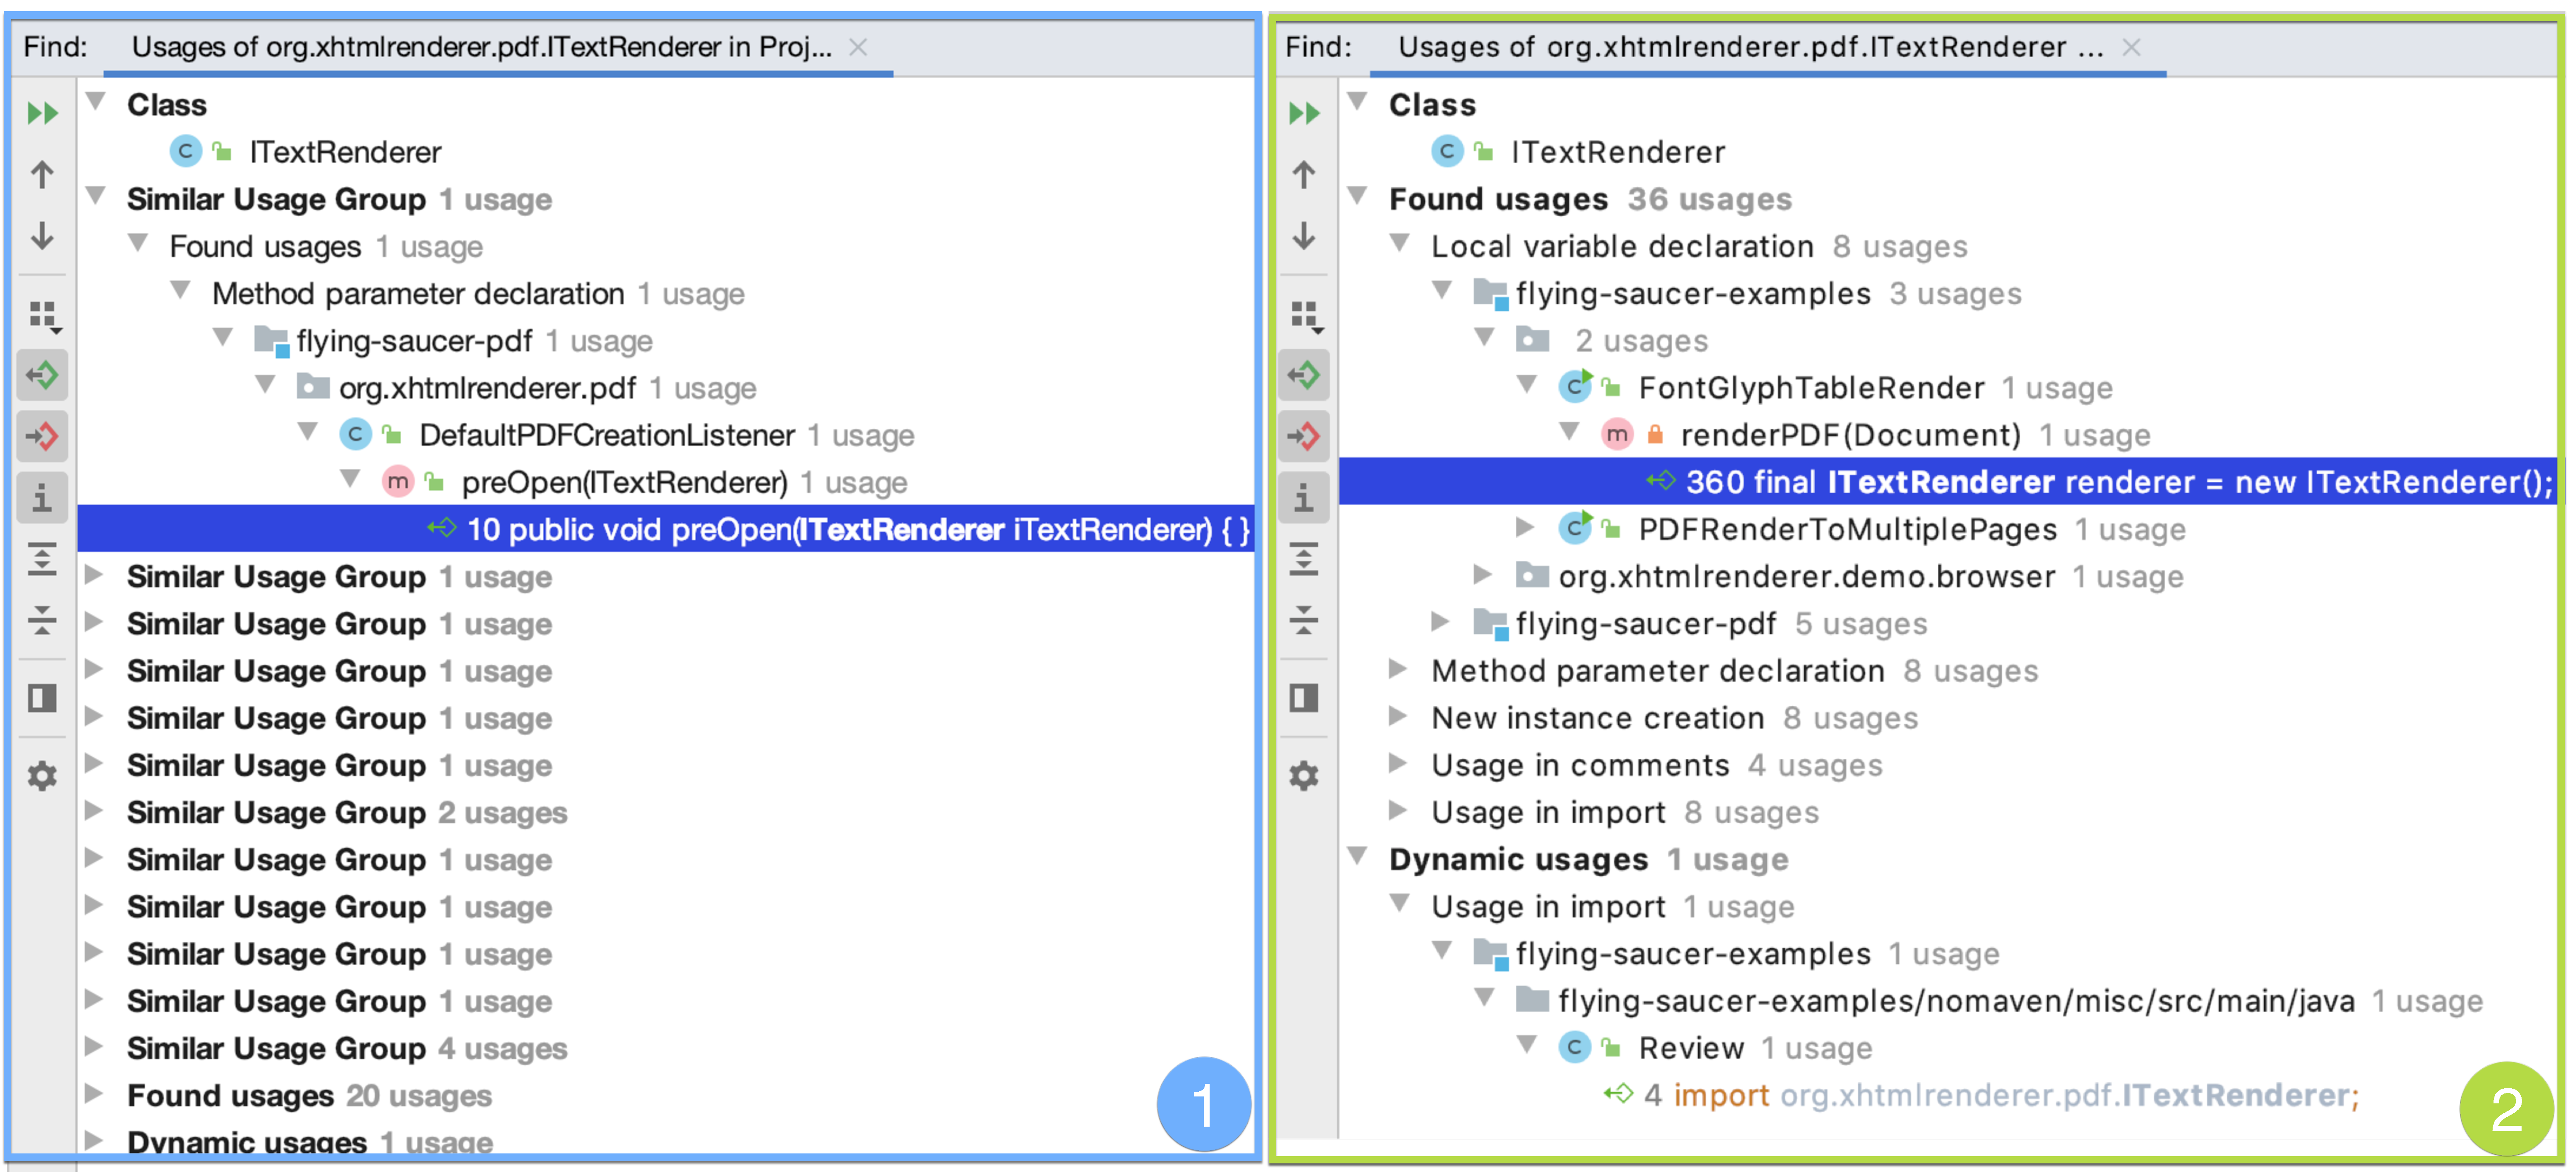
\includegraphics [width=\textwidth,keepaspectratio,clip]{figures/compare}
    \caption{In the blue rectangle number 1 screenshot the interface of Find Distinct Usages an the in the number 2 the regular Find Usages are depicted. }
\label{fig:compare}
\end{figure*}

\subsection{Results}
To investigate the productivity of Find Distinct Usages, we measure the completion time of the task. Participants in the experimental group completed that task in a median of 21.5 minutes and 33 minutes in the control group. \par

A qualitative data might be useful is behaviors of developers. We observed the behaviors of developers and labeled them to find a pattern from their activities while they were working on the task. The bellow behaviors are common between both control and experimental group. The reason that they had many common behaviors was the user interface for our tool and regular Find Usages tool was similar. \par

Several sequential using of Find Usages feature is misleading. After participants selected a usage, they clicked on that usages and opened the class that contained that usage. In that class, they use another Find Usages on other methods. Sometimes they called Find Usages several times, and they forgot the call graph and got lost. So they left the usage and came back to the list of results. After that, they chose another use. \par

Inline Find Usages might be more useful than seeing results in a separate result window. IntelliJ IDEA has inline Find Usages by pressing control on the keyboard and clicking by mouse on the method that shows a list of usages. In this approach, developers do not go to a separate result window. The result of this approach has a better abstraction. One developer from control group that used this approach she completed the task in 17 minutes. Seventeen minutes was the second minimum of time among the completion time of all participants. Another developer that used this approach was from the experimental group. He completed the task in 13 minutes, which was the lowest among 12 participants. \par

Usages that they accept primitive type like integer are easier to understand than usages they have variable in their input arguments. Results of Find Usages that have a variable, not primitive types, were forcing developers to open the class and read the class to understand the usage. Clicking on the usage an going to another window was required in some cases.\par

Participants did not skim all results of Find Usages in the beginning. They read result of usages sequentially. They start from the first result in the list then go through the other. Find Usages window of IntelliJ IDEA expand and open the first usage, it might be a reason.\par

There was a pattern for productive participants, 1) They utilized Find Usages with Find In Path features for understanding the codebase.  2) Before start reading usages, they expand usages and skimmed the list of usages. After that decided to go through the best usage that might help them. \par

At the end of the study, we interviewed all participants and asked them to tell us about their experience. One participant told us that several sequential using of Find Usages feature is misleading.
\begin{quote} "I was getting lost when I was using nested [several sequential] Find Usages for understand codebase." - (P10)\end{quote}

 An interesting usability issue that P10 and P13 had with regular Find Usages was the number in the result that shows the line of the statement. They told us they thought this number is the frequency of repeating that statement.\par
 
We received feedback about the grouping of usages in our approach. Find Distinct Usages approach used a similar name for all groups in the list of result.It was confusing for 2 of participants (P12 and P14). They suggested us to change the naming convention. Since the name of all groups was similar (see Figure.~\ref{fig:compare}) they were curious how we grouped the usages.\par

Also we asked them give us any suggestion that might be useful. They gave us couple of suggestion. The interesting one was P10 told us if they have Call Graphs in combination with Find Usages might be useful. 



% *************************Limitation********************************************************************
\section{Limitation And Threats To Validity}
Our study had several limitations and potential threats to the internal and external validity of the results. \par  

In selecting a task, we sought to identify a task that is representative of a typical large codebase that contains many usages for methods. Smaller or Larger codebase may involve more complex usages where individual behaviors are more challenging to identify. \par 

Second threat is Find Distinct Usages approach is dependent on IDE and language. It is not clear if we use it on other IDEs or other languages, the result might be different.\par 

% *************************Discussion********************************************************************
\section{Discussion}
Our exploratory study showed there exist challenges in Find Usages feature of IntelliJ IDEA. We designed an approach and implement a plugin on top of Find Usages feature of IntelliJ IDEA to fix the issues. Our approach utilize AST diffs of usages for grouping similar usages in one group. The result of controlled experiment showed our approach could decrease 35\% of time completion of implementation a simple logic in a large codebase.

The approach that we used for grouping the usage was a naive approach to clustering that we took due to time constraints preventing us from better understanding the IntelliJ SDK. In the future, we hope to re-implement the usage grouping with merging as part of an agglomerate clustering approach. Also, We can work on scalability and response time of the plugin \par

A couple of participants complaint about the naming convention of groups. Names were similar. In future, we must change it to more readable names.\par

IntelliJ IDEA by default open and extend the first usages in the list of result. Another issue that we observed was If Find Usages feature expands all usage by default that might be more useful for developers.\par

IntelliJ IDEA had inline Find Usages feature, which looks great. We did not think about it. Nevertheless, we guess developers who use the inline Find Usages might be more productive. In the future, we might compare them. \par

In future work this should either be picked based on trying out different thresholds on different projects or probably better allowing it to be configured by a menu option as part of the IDE plugin. Choosing the similarity threshold here for describing similar code, is also familiar to choosing a K when doing K-means, which depends highly on the data-set that K-means is applied to. Picking a good default threshold would be future work, but for now the best approach would probably be to set it as an option via a menu.

% *************************Conclusion********************************************************************
\section{Conclusion}
Developers have difficulties in understanding the context of how various internal classes, objects, or methods are used in the codebase. We sought to better understand these challenges by conducting a think-aloud user study with 6 participants. The results of the think-aloud experiment highlighted that developers spend considerable time learning to use internal code artifacts. The result also showed developers use the Find Usages/References feature of IDEs to understand code by example. The results of Find Usages can be long tail of results that developers find difficulty mentally parsing. We also found that find usage/reference results' would contain duplicate examples in disparate locations in the UI, adding to the difficulty of parsing. Based on the think-aloud study. We designed and implemented a plugin for IntelliJ IDEA that manipulated result of Find Usages and grouped them based on their similarity. After that, we conducted a controlled experiment with 12 more participants to evaluate our approach. Results showed that this aggregation of distinct examples save 35\% times of developers..


% \section*{Acknowledgment}
% % [TODO]: mention Dr. Jon Bell. He helped us in first ideation part of the paper.
% acknowledgments in the unnumbered footnote on the first page.

\bibliographystyle{IEEEtran}
\bibliography{FUU}



\end{document}
